\section{Динамическая байесова сеть}

Байесова сеть — графическая вероятностная модель, представляющая собой множество переменных и их вероятностных зависимостей. Например, байесова сеть может быть использована для вычисления вероятности того, чем болен пациент по наличию или отсутствию ряда симптомов, основываясь на данных о зависимости между симптомами и болезнями.

Формально, байесова сеть — это направленный ациклический граф, каждой вершине которого соответствует случайная переменная, а дуги графа кодируют отношения условной независимости между этими переменными. Вершины могут представлять переменные любых типов, быть взвешенными параметрами, скрытыми переменными или гипотезами. Существуют эффективные методы, которые используются для вычислений и обучения байесовых сетей. Если переменные байесовой сети являются дискретными случайными величинами, то такая сеть называется дискретной байесовой сетью. Байесовы сети, которые моделируют последовательности переменных, называют динамическими байесовыми сетями. Байесовы сети, в которых могут присутствовать как дискретные переменные, так и непрерывные, называются гибридными байесовыми сетями. 

\subsection{Определение}
Если дуга выходит из вершины $A$ в вершину $B$, то $A$ называют родителем $B$, а $B$ называют потомком $A$. Если из вершины $A$ существует ориентированный путь в другую вершину $B$, то $B$ называется потомком $A$, а $A$ называется предком $B$. Множество вершин-родителей вершины $V_i$ обозначим как $parents(V_i) = PA_i$.

Направленный ациклический граф G называется байесовой сетью для вероятностного распределения $P(v)$, заданного над множеством случайных переменных $V$, если каждой вершине графа поставлена в соответствие случайная переменная из $V$, а дуги в графе удовлетворяют условию (марковское условие ~\cite{m_chain}): любая переменная $V_i$ из $V$ должна быть условно независима от всех вершин, не являющихся ее потомками, если заданы (получили означивание, обусловлены) все ее прямые родители $PA_i$ в графе $G$, то есть $\forall V_i \in V$ справедливо: $P(v_i|pa_i,s) = P(v_i|pa_i)$, где $v_i$ — значение $V_i; S$ — множество всех вершин, не являющихся потомками $V_i$; $s$ — конфигурация $S$; $pa_i$ — конфигурация $PA_i$.

Тогда полное совместное распределение значений в вершинах можно удобно записать в виде декомпозиции (произведения) локальных распределений:

\begin{equation}
	P(V_1,...,V_n)=\prod_{i=1}^{n}P(V_i|parents(V_i))
\end{equation}

Если у вершины $V_i$ нет предков, то её локальное распределение вероятностей называют безусловным, иначе условным. Если вершина - случайная переменная получила означивание (например, в результате наблюдения), то такое означивание называют свидетельством. Если значение переменной было установлено извне (а не наблюдалось), то такое означивание называется вмешательством.

\subsection{Цепь маркова}
Цепь Маркова — последовательность случайных событий с конечным или счётным числом исходов, характеризующаяся тем, что при фиксированном настоящем будущее независимо от прошлого.

Процесс в каждый момент времени находится в одном из $n$ состояний. 
При этом, если он находится в состоянии с номером $i$, то он перейдет в состояние $j$ с вероятностью $p_{ij}$.
Матрицу $P=||p_{ij}||$ называют матрицей переходов.

На матрицу переходов накладываются следующие условия: 

\begin{subequations}
\begin{align}
  p_{ij}>0 \\
  \forall i \sum_j p_{i,j}=1
\end{align}
\end{subequations}

Такая матрица называется стохастической.

Марковскую цепь можно представить в виде графа, в котором вершины — это состояния процесса, а ребра — переходы между состояниями, и на ребре из $i$ в $j$ написана вероятность перехода из $i$ в $j$, то есть $p_{ij}$. 

Марковскую цепь в любой момент времени $t$ можно охарактеризовать вектором-строкой $c_t$ — распределением вероятностей по состояниям цепи ($c_{ti}$ — вероятность цепи в момент времени $t$ быть в состоянии $i$). 

Если $c_i$ — текущее распределение вероятностей, то можно узнать распределение на следующем шаге, умножив вектор на матрицу перехода: 

\begin{equation}
  c_{i+1}=c_i P
\end{equation}

Из ассоциативности произведения матриц следует, что для того, чтобы узнать распределение вероятностей через $t$ шагов, нужно умножить $c_i$ на матрицу перехода, возведённую в степень $t$: 

\begin{equation}
  c_{i+t}=c_i P_t
\end{equation}

Для марковской цепи иногда задают начальное распределение $c_0$, хотя во многих классах марковских цепей распределение по прошествии большого периода времени от него не зависит (такое распределение называют предельным). 

\subsection{EM - алгоритм}

EM-алгоритм (Expectation-maximization (EM) algorithm) — алгоритм, используемый в математической статистике для нахождения оценок максимального правдоподобия параметров вероятностных моделей, в случае, когда модель зависит от некоторых скрытых переменных. Каждая итерация алгоритма состоит из двух шагов. На E-шаге (expectation) вычисляется ожидаемое значение функции правдоподобия, при этом скрытые переменные рассматриваются как наблюдаемые. На M-шаге (maximization) вычисляется оценка максимального правдоподобия, таким образом увеличивается ожидаемое правдоподобие, вычисляемое на E-шаге. Затем это значение используется для E-шага на следующей итерации. Алгоритм выполняется до сходимости.

Пусть \textbf{X} — некоторые из значений наблюдаемых переменных, а \textbf{T} — скрытые переменные. Вместе \textbf{X} и \textbf{T} образуют полный набор данных. Вообще, \textbf{T} может быть некоторой подсказкой, которая облегчает решение проблемы в случае, если она известна. Например, если имеется смесь распределений, функция правдоподобия легко выражается через параметры отдельных распределений смеси.

Положим $p$, — плотность вероятности (в непрерывном случае) или функция вероятности (в дискретном случае) полного набора данных с параметрами $\theta: p(X,T|\theta)$. Эту функцию можно понимать как правдоподобие всей модели, если рассматривать её как функцию параметров $\theta$. Заметим, что условное распределение скрытой компоненты при некотором наблюдении и фиксированном наборе параметров может быть выражено так:

\begin{equation}
	P(T|X,\theta)=\frac{p(X|T,\theta)}{p(X|\theta)}=\frac{p(X|T,\theta)p(T|\theta)}{\int p(X|T,\theta)p(T|\theta)dT}
\end{equation}
\par
используя расширенную формулу Байеса и формулу полной вероятности. Таким образом, нам необходимо знать только распределение наблюдаемой компоненты при фиксированной скрытой $p(X|T,\theta)$ и вероятности скрытых данных $p(T|\theta)$.

EM-алгоритм итеративно улучшает начальную оценку $\theta_0$, вычисляя новые значения оценок $\theta_1$, $\theta_2$, и так далее. На каждом шаге переход к $\theta_{n+1}$, от $\theta_n$, выполняется следующим образом:

\begin{equation}
	\theta_{n+1}=arg \max_{\theta} Q(\theta)
\end{equation}
\par
где $Q(\theta)$ — матожидание логарифма правдоподобия. Другими словами, мы не можем сразу вычислить точное правдоподобие, но по известным данным ($X$) мы можем найти апостериорную оценку вероятностей для различных значений скрытых переменных $T$. Для каждого набора значений $T$ и параметров $\theta$ мы можем вычислить матожидание функции правдоподобия по данному набору $X$. Оно зависит от предыдущего значения $\theta$, потому что это значение влияет на вероятности скрытых переменных $T$.

$Q(\theta)$ вычисляется следующим образом:

\begin{equation}
	Q(\theta) = E_T[\log p(X,T|\theta)|X]
\end{equation}


\subsection{Алгоритм построения динамической байесовой сети}

Для решения задачи кликов, построим математичепскую модель. Будем предполагать, что пользователь просматривает документы последовательно сверху вниз, при этом производя клики на документы, которые его заинтересовали. Ввод нового запроса будем ассоциировать с новой сессией. Это довольно схоже с каскадной моделью кликов.~\cite{cascade_click_book}

Динамическая байесова сеть представляет из себя марковскую цепь, представленную на ~\ref{dbn-picture}. Это вероятностная модель, основанная на действиях пользователей. В ней рассматриваются сессии целиком. В этом случае для каждой сессии мы можем построить марковскую цепь. Для i-того документа имеем $C_i$ - клик пользователя на документ - наблюдаемый параметр, также набор скрытых переменных, которые описаны ниже.	

Данная модель определяется следующими параметрами(представленные ниже параметры могут принимать значения ${0;1}$): 
\begin{itemize}
	\item $A_i$ - привлекательность i-того документа для пользователя. 
	\item $E_i$ - параметр, определяющий посмотрел ли пользователь i-тый документ. 
	\item $S_i$ - удовлетворенность документом.
\end{itemize}

С учетом этого, мы можем записать полную вероятностную модель:

\begin{subequations}
\begin{align}
	A_i=1,E_i=1 \iff  C_i=1 \\
	P(A_i)=a_u \\
	P(S_i=1|C_i=1)=s_u \\
	C_i=0 \implies S_i=0 \\
	S_i=1 \implies E_{i+1}=0 \\
	P(E_{i+1}=1|E_i=1,S_i=0)=\gamma \\
	E_i=0 \implies E_{i+1}=0 
\end{align}
\end{subequations}

\begin{figure}
  \centering
  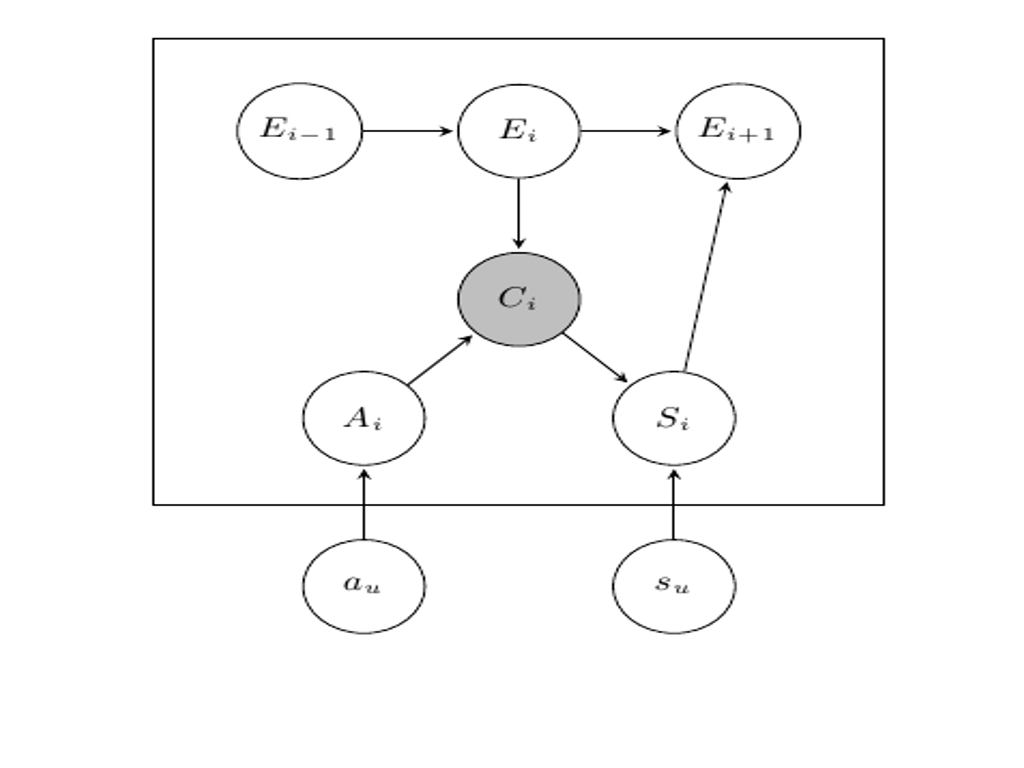
\includegraphics[width=0.9\textwidth]{images/dbn.png}
  \caption{Динамическая байесова сеть\label{dbn-picture}}
\end{figure}

Предполагается, что пользователь произвел клик по документу, если он его исследовал($E_i=1$) и документ его привлек($A_i=1$). Кроме этого, вероятность того, что пользователя привлек документ равняется $a_u$. Также, введен параметр удовлетворенности документом($S_i$). Предполагается, что если пользователь на произвел клик по документу($C_i=0$), то документ был неинформативным($S_i=0$). Иначе, документ считается информативным и пользователь не будет просматривать следующий документ ($S_i=1 \implies E_{i+1}=0$). Если документ оказался неинформативным, то пользователь может с какой-то вероятностью $\gamma$ продолжить сессию $P(E_{i+1}=1|E_i=1,S_i=0)=\gamma$. Т.к. мы предполагаем что данная модель последовательна, то $E_i=0 \implies E_{i+1}=0$.

Определим понятие релевантности документа:
\begin{equation}
	r_u=P(S_i=1|E_i=1)\\
	   =P(S_i=1|C_i=1)P(C_i=1|E_i=1)\\
	   =a_u s_u
\end{equation}


Решение и нахождение релевантности документов зависит от параметра $\gamma$. При $\gamma =1$ нам точно известно, что пользователь остановится после того, как его не удовлетворил документ $i$. Данный алгоритм приведен ниже:

\begin{algorithm}
  \caption{Простой алгоритм нахождения релевантности}
  \label{overall-boosting-algorithm}
  \begin{enumerate}
  \item Инициализировать переменные $a_{u}^{N},a_{u}^{D},s_{u}^{N},s_{u}^{D}$ в значение 0, для всех url ассоциированых для текущего запроса.
  \item Для каждой сессии:
    \begin{enumerate}
      \item Для всех u выше или раано последней кликнутой url в данной сессии:
      	\begin{enumerate}
      		\item $a_{u}^{D}=a_{u}^{D}+1$
      	\end{enumerate}
      \item Для всех url, по которым был произведен клик:
      	\begin{enumerate}
      		\item $a_{u}^{N}=a_{u}^{N}+1$
      		\item $s_{u}^{D}=s_{u}^{D}+1$
      	\end{enumerate}
      \item $s_{u}^{N}=s_{u}^{N}+1$ для последней клинутой url
    \end{enumerate}
    \item для всех url $u$ :
    	\begin{enumerate}
    		\item $a_u=(a_{u}^{N}+\alpha_a)/(a_{u}^{D}+\alpha_a+\beta_a)$
    		\item $s_u=(s_{u}^{N}+\alpha_s)/(s_{u}^{D}+\alpha_s+\beta_s)$
    	\end{enumerate}
  \end{enumerate}
\end{algorithm}

Построение алгоритма EM производится с помощью двух шагов : E и M.
На шаге М, нам даны постериорные распределения скрытых параметров $Q(A_{i}^{j},Q(s_{i}^{j}$. Пересчитываем параметры $a_u,s_u$:

\begin{subequations}
\begin{align}
	a_u=arg \max_a \sum_{j=1}^{N}\sum_{i=1}^{M}I(d_i=u) \nonumber \\
	(Q(A_{i}^{j}=0)\log(1-a)+Q(A_{i}^{j}=1)\log(a))+\log P(a) \\
	s_u=arg \max_s \sum_{j=1}^{N}\sum_{i=1}^{M}I(d_i=u) \nonumber \\
	(Q(S_{i}^{j}=0)\log(1-s)+Q(S_{i}^{j}=1)\log(s))+\log P(s)
\end{align}
\end{subequations}

На шаге Е, по найденным параметрам пересчитываем постериорные вероятности  $Q(A_{i}^{j},Q(s_{i}^{j}$.

\begin{subequations}
\begin{align}
	Q(A_{i}^{j})=P(A_{i}^{j}|C^j,a_u,s_u,\gamma)
	Q(S_{i}^{j})=P(A_{i}^{j}|C^j,a_u,s_u,\gamma)
\end{align}
\end{subequations}

Для ЕМ алгоритма введем дополнительные параметры $\alpha_i(e),\beta_i(e)$:


\begin{subequations}
\begin{align}
	\alpha_i(e)=P(C_{1}^{j},...,C_{i-1}^{j}|E_i=e) \\
	\beta_i(e)=P(C_{i}^{j},...,C_{M}^{j}|E_i=e)
\end{align}
\end{subequations}

Данные параметры мы можем вычислить рекурсивно по правилам:

\begin{subequations}
\begin{align}
	\alpha_{i+1}(e)=\sum_{e \in {0,1}}\alpha_i(e)P(E_{i+1}=e,C_i|E_i=e)\\
	\beta_{i-1}(e)=\sum_{e \in {0,1}}\beta_i(e)P(E_{i}=e,C_{i-1}|E_{i-1}=e)
\end{align}
\end{subequations}

В свою очередь, $P(E_{i+1}=e,C_i|E_i=e)$ вычисляется следующим образом:

\begin{subequations}
\begin{align}
	P(E_{i+1},C_i|E_i)=\sum_{s \in {0,1}}P(E_{i+1}|S_i=s,E_i)P(S_i=s|C_i)P(C_i|E|i)
\end{align}
\end{subequations}

С учетом правил, приведенных выше можно найти релевантности документов. Структура алгоритма ЕМ приведена на ~\ref{em-picture}.

\begin{figure}
  \centering
  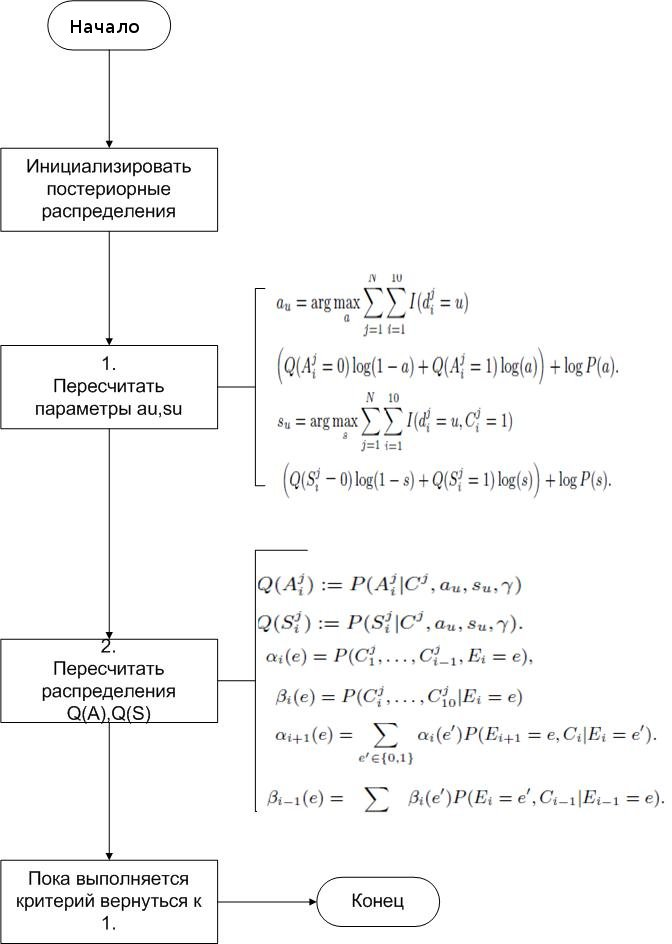
\includegraphics[width=0.9\textwidth]{images/em_new.jpg}
  \caption{Схема ЕМ алгоритма\label{em-picture}}
\end{figure}

\subsection{Выводы}
 
 Данный алгоритм является хорошей опорой для разработки алгоритмов ранжирования. Используемые данные(релевантности документов) будут использованы как конечные цели в тренеровки градиентного бустинга на основе деревьев решений.

К плюсам данного алгоритма можно отнести его относительную легкость построения, быструю сходимость и возможность корректировки результатов с приходом новых данных.

\newpage